\chapter{Processi}
\begin{defn}[Processo]
Un processo è un programma in esecuzione.
\end{defn}
L'attività corrente del processo è rappresentata dal valore del \textbf{program counter} e dal contenuto dei registri.
\vspace*{0.01\textheight}
Il layout della memoria è diviso in varie parti:
\begin{itemize}
  \item \textbf{Text Section:} codice eseguibile.
  \item \textbf{Data Section:} variabili globali.
  \item \textbf{Heap Section:} memoria allocata dinamicamente durante il tempo di esecuzione.
  \item \textbf{Stack Section:} spazio dei dati temporaneo quando vengono chiamate le funzioni.
\end{itemize}

\begin{figure}[!htb]
    \centering
    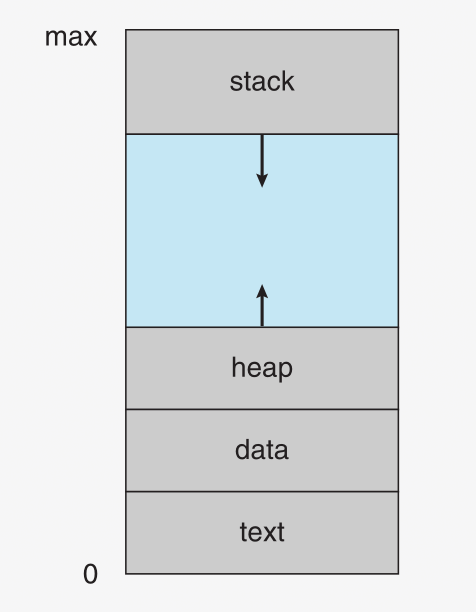
\includegraphics[width=0.3\linewidth]{Images/process/memoria.png}
    \caption{Layout Memoria.}
\end{figure}

La dimensione della sezione Data e della sezione Text sono fissate e non possono cambiare, invece, la dimensione dello Stack e dell'Heap può aumentare o diminuire dinamicamente. \\ 
Per esempio, per ogni funzione viene dichiarato un \textbf{Record di Attivazione}, con tutte i dati della funzione e viene pushato e tolto dallo stack. Invece, l'Heap può crescere in base alla memoria allocata. \\ 
Anche se queste due aree della memoria crescono una verso l'altra, il sistema operativo ha il compito di non farli mai accavallare.

\section{Stato dei Processi}
Durante la sua esecuzione, un processo può cambiare stato. Un processo può avere cinque stati differenti:
\begin{enumerate}
  \item \textbf{New:} il processo è stato creato.
  \item \textbf{Running:} le istruzione vengono eseguite.
  \item \textbf{Waiting:} il processo sta aspettando l'accadimento di alcuni eventi.
  \item \textbf{Ready:} il processo sta aspettando di essere assegnato a un processore.
  \item \textbf{Terminated:} il processo ha finito l'esecuzione.
\end{enumerate}

\begin{figure}[!htb]
    \centering
    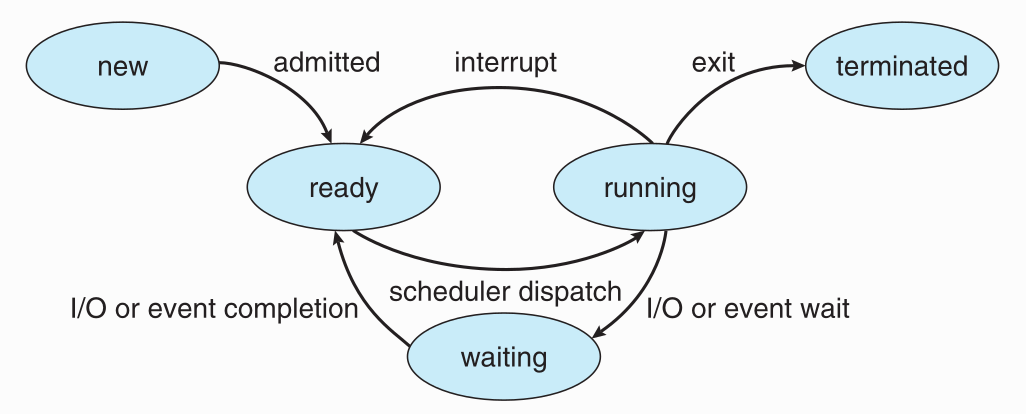
\includegraphics[width=0.6\linewidth]{Images/process/stato.png}
    \caption{Stati Possibili di un Processo.}
\end{figure}

\section{Process Control Block (PCB)}
Ogni processo, all'interno del sistema operativo, è reppresentato da un \textbf{Process Control Block} o \textbf{Task Control Block}. Al suo interno sono contenuti tutte le informazioni associate a un processo.

\begin{figure}[!htb]
    \centering
    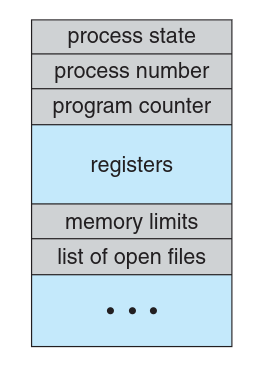
\includegraphics[width=0.2\linewidth]{Images/process/pcb.png}
    \caption{PCB.}
\end{figure}

Nello specifico, vengono specificate le seguenti informazioni:
\begin{itemize}
  \item \textbf{Process State:} indica lo stato del processo.
  \item \textbf{Program Counter:} contiene l'indirizzo della prossima istruzione da eseguire.
  \item \textbf{CPU Registers:} contiene il tipo, il numero e lo stato dei registri usati.
  \item \textbf{CPU-Scheduling Information:} include i parametri per lo scheduling.
  \item \textbf{Memory-Managment Information:} pagine o tabelle di memoria e altre informazioni.
  \item \textbf{Accounting Informaztion:} quantità di tempo di CPU e tempo reale usato, job or process number, limiti di tempo e altre informazioni.
  \item \textbf{I/O Status Information:} lista dei dipositivi I/O parti, lista dei file aperti e altro.
\end{itemize}

All'interno dei sistemi Linux ogni PCB è reppresentato dalla structure \texttt{task\_struct}, che si trova nel file \texttt{<include/linux/sched.h>} del kernel linux.
\begin{clang}[struct task\_struct]
struct task_struct {
  long state;                     /* state of the process */
  struct sched_entity se;         /* scheduling information */
  struct task_struct *parent;     /* this process’s parent */
  struct list_head children;      /* this process’s children */
  struct file_struct *files;      /* list of open files */
  struct mm_struct *mm;           /* address space */
}
\end{clang}

Si può notare che all'interno della struct, oltre ai file aperti, lo stato del processo e altre informazioni,
è presente pure il puntatore a una coda con i processi figli e uno che punta al processo padre. \\
\vspace*{0.01\textheight}
Inoltre, sempre nei sistemi operativi Linux, sono presenti altri stati oltre a quelli classici:
\begin{itemize}
  \item \textbf{TASK\_INTERRUPTIBLE:} il task sta aspettando, può essere interrotto da un segnale.
  \item \textbf{TASK\_UNINTERRUPTIBLE:} il task sta aspettando e non può essere interrotto da un segnale.
  \item \textbf{EXIT\_ZOMBIE:} il processo è terminato ma le risorse devono ancora essere deallocate.
  \item \textbf{EXIT\_DEAD:} il processo è terminato e le risorse sono state deallocate.
  \item \textbf{TASK\_STOPPED:} il task è stato interrotto da una azione del terminale (\texttt{CTRL + Z}).
  \item \textbf{TASK\_TRACED:} il task è seguito da un altro processo per un esecuzione passo passo.
\end{itemize}

\begin{clang}[/include/linux/sched.h]
/* Used in tsk->__state: */
#define TASK_RUNNING 0x00000000
#define TASK_INTERRUPTIBLE 0x00000001
#define TASK_UNINTERRUPTIBLE 0x00000002
#define __TASK_STOPPED 0x00000004
#define __TASK_TRACED 0x00000008
#define EXIT_DEAD 0x00000010
#define EXIT_ZOMBIE 0x00000020
#define EXIT_TRACE (EXIT_ZOMBIE | EXIT_DEAD)

/* Used in tsk->__state again: */
#define TASK_PARKED 0x00000040
#define TASK_DEAD 0x00000080
#define TASK_WAKEKILL 0x00000100
#define TASK_WAKING 0x00000200
#define TASK_NOLOAD 0x00000400
#define TASK_NEW 0x00000800
\end{clang}

\section{Scheduling dei Processi}
Per una CPU con un solo core, non potrà mai esserci più di un processo in esecuzione. Invece, in caso di una archiettura multicore, i processi dovranno essere schedulati e aspettare un core libero.
Il numero di processi in memoria è detto \textbf{grado di multiprogrammazione}. 

\subsection{Code di Scheduling}
Quando i processi entro nel sistema, vengono inseriti in una coda, la \textbf{Ready Queue}. 
Questa coda è una linked-list, l'intestazione contiene il puntatore al primo PCB e ogni altro PCB contiene il puntatore al prossimo task della coda. \\ 
Esistono anceh altre code, nello specifico, se per esempio un processo deve fare delle lunghe operazioni di I/O, allora il processo che dovrà aspettare verrà messo nella \textbf{Wait Queue}. \\
Un ottimo modo per rappresentare lo scheudling di un processo è tramite un diagramma. \\ 
Per prima cosa, un processo viene inserito nella coda ready dove aspettare di essere eseguito, successivamente,in base alla circostanze, può essere messo nel coda di wait o di nuovo nella coda di ready.

\begin{figure}[!htb]
    \centering
    \begin{subfigure}{0.48\linewidth}
        \centering
        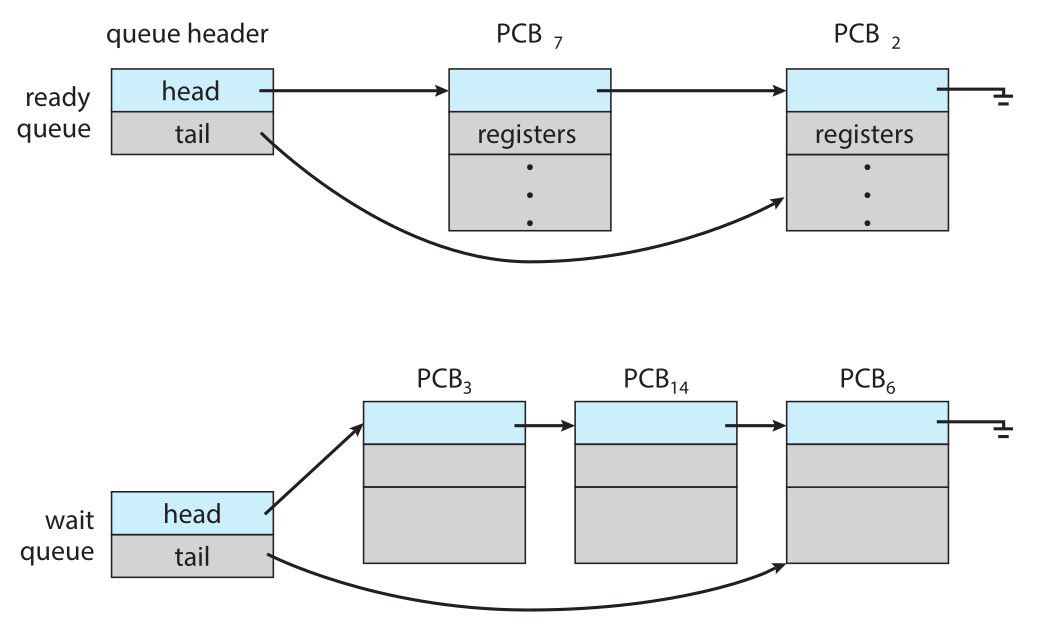
\includegraphics[width=\linewidth]{Images/process/queue.png}
        \caption{Code Ready e Wait.}
    \end{subfigure}
    \hfill
    \begin{subfigure}{0.48\linewidth}
        \centering
        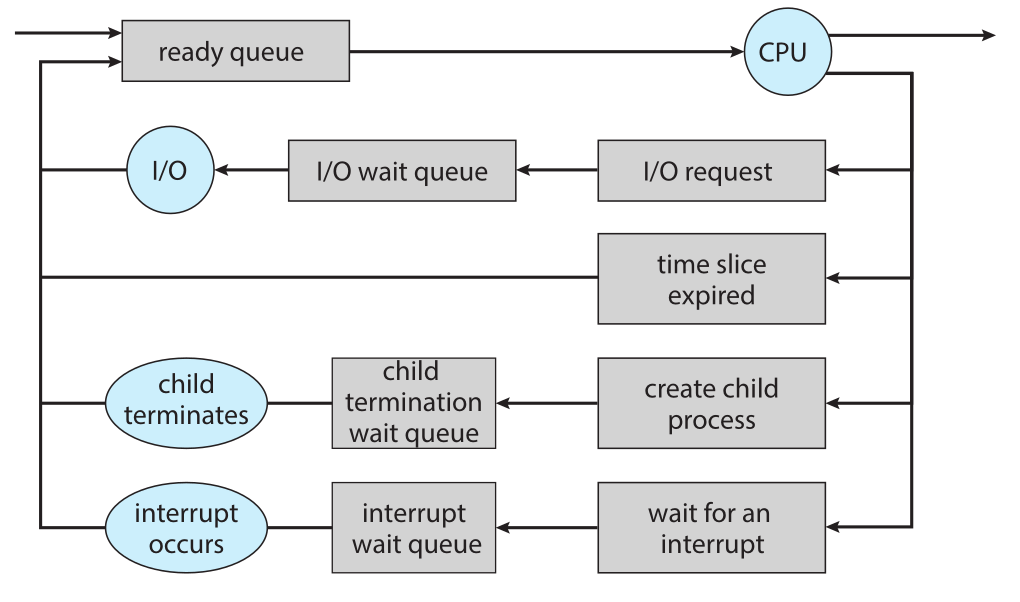
\includegraphics[width=\linewidth]{Images/process/sched.png}
        \caption{Diagramma dello Scheudling di un Processo.}
    \end{subfigure}
\end{figure}

Questo ciclo viene eseguito finchè il processo non termina. In tal caso, se il processo ha finito la sua esecuzione, verrà rimosso da ogni coda e le risorse del PCB verranno deallocate.

\subsection{Cambio di Contesto}
In sistemi moderni general-purpose, la frequenza di interrupt che richiedono una routine del kernel per essere gestiti, può essere elevata. 
Ogni volta che accade, deve essere salvato il \textbf{contesto} del processo in esecuzione sul core, per poterlo ripristinare successivamente. 
Tutti questi dati sono salvati all'interno del PCB, permettendo quindi due azioni: \textbf{save state} e \textbf{restore state}. \\ 

\begin{figure}[!htb]
    \centering
    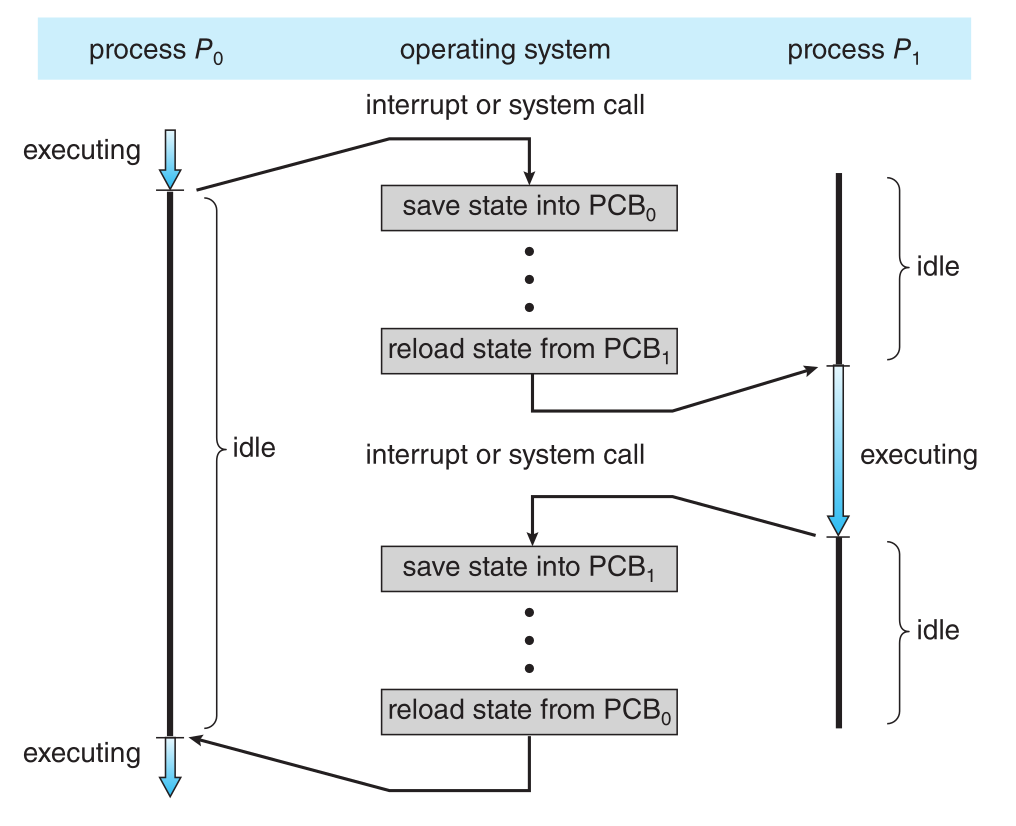
\includegraphics[width=0.5\linewidth]{Images/process/switch.png}
    \caption{Context Switch.}
\end{figure}

Il tempo per il cambio di contesto è puro overhead, dato che il sistema non fa nulla di utile in questi millisecondi. 
Più è alta la complessità del sistema e del PCB più tempo sarà necessario. La velocità delle memorie può aiutare a ridurre il tempo di cambio di contesto. \\ 

\section{Creazioni di Processi}
I processi possono creare a loro volta altri processi figli, che a loro volta ne possono creare altri. Questo porta alla creazione di un labero dei processi.
Ogni processo è indificato dal \textbf{Process Identifier} (\textbf{PID}), che di solito è un integer. Alla creazione, ci possono essere diverse opzioni:
\begin{itemize}
  \item \textbf{Condivisione delle Risorse:} 
  \begin{itemize}
    \item Genitore e figlio condividono le stesse risorse.
    \item Il figlio condivide un sottoinsieme delle risorse del genitore.
    \item Genitore e figlio non condividono nessuna risorsa.
  \end{itemize}
  \item \textbf{Esecuzione:}
  \begin{itemize}
    \item Il processo figlio e quello genitore eseguono contemporaneamene.
    \item Il genitore aspetta che il figlio termini.
  \end{itemize}
  \item \textbf{Spazio di Indirizzamento:}
  \begin{itemize}
    \item Il figlio è una copia duplicata del padre.
    \item Viene caricato un altro programma all'interno del figlio.
  \end{itemize}
\end{itemize}

\subsection{System Calls \texttt{fork()} e \texttt{exec()}}
Nei sistemi Linux, per creare un nuovo processo può essere usata la funzione \texttt{fork()}. 
Con questa istruzione, viene creato un nuovo processo figlio, con lo stesso spazio di indirizzamento del padre. 
Al suo interno può essere eseguito anche un altro programma, tramite la funzione \texttt{exec()}. \\
I due processi inizialmente eseguono contemporaneamene, nello specifico, il processo figlio avrà un valore di ritorno di \texttt{fork()} con valore uguale a zero, invece, il genitore avrà un valore diverso da zero.

\begin{clang}[Esempio di utilizzo di fork() e exec()]
#include <sys/types.h>
#include <stdio.h>
#include <unistd.h>

int main()
{
  pid_t pid;
  
  /* fork a child process */
  pid = fork();
  if (pid < 0) { /* error occurred */
    fprintf(stderr, "Fork Failed");
  return 1;
  }
  else if (pid == 0) { /* child process */
    execlp("/bin/ls","ls",NULL);
  }
  else { /* parent process */
    /* parent will wait for the child to complete */
    wait(NULL);
    printf("Child Complete");
  }
}

return 0;
\end{clang}

\subsection{Terminazione dei Processi}
Normalmente, un processo esegue tutte le istruzioni e poi chiede al sistema operativo di interromperlo con la system call \texttt{exit()}. 
In questo caso, le risorse sono deallocate e viene ritornato un valore al genitore che sta aspettando con la system call \texttt{wait()}. \\ 
In alcuni casi, è possibile terminare anche con la system call \texttt{abort()}. \\ 
\vspace*{0.01\textheight}
Se viene terminato un processo genitore, allora anche tutti i figli verranno terminati, altrimenti si possono verficare situazioni problematiche:
\begin{itemize}
  \item Se il genitore non usa l'istruzione \texttt{wait()}, allora i processi figli saranno chiamati \textbf{zombie}.
  \item Se il genitore si interrompe prima di chiamare l'istruzione \texttt{wait()}, allora i processi figli saranno \textbf{orfani}.
\end{itemize}

\newpage
\section{Comunicazione fra Processi}
All'interno di un sistema, i processi possono essere indipendenti oppure possono cooperare. 
In quest'ultimo caso, necessitano di un modo per comunicare, ossia una \textbf{Interprocess Comunication} (\textbf{IPC}). \\ 
Le modalità possono essere due: \textbf{shared memory} o \textbf{message passing}.

\begin{figure}[!htb]
    \centering
    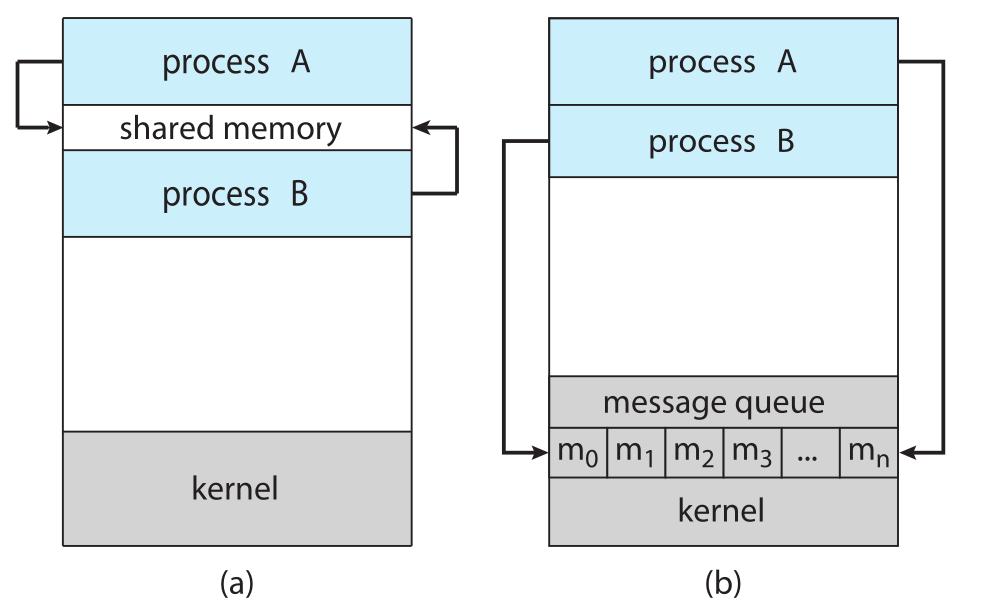
\includegraphics[width=0.5\linewidth]{Images/process/comunication.png}
    \caption{Diverse Modalità di Comunicazione.}
\end{figure}


\begin{intuition}[Problema Produttore-Consumatore]
Processo \textbf{produttore} produce informazione e il processo \textbf{consumatore} la consuma. \\
Può avere due variazioni:
\begin{itemize}
  \item \textbf{Unbounded-Buffer:} non c'è alcun limite pratico alla dimensione del buffer. Il produttore non attende mai.
    Il consumatore attende se non c'è alcun buffer da consumare.
  \item \textbf{Bounded-Buffer:} presuppone che vi sia una dimensione fissa del buffer. Il produttore deve attendere se tutti i buffer sono pieni. 
    Il consumatore attende se non vi è alcun buffer da consumare.
\end{itemize}
\end{intuition}

\subsection{Shared Memory}
Un modo per comunicare fra processi è creare un'area condivisa in cui vengono scritte e lette informazioni. \\
Il controllo è lasciato ai processi utenti e necessita di un meccanismo di sincronizzazione per condinare l'accesso alla memoria. \\ 
\vspace*{0.01\textheight}
Per esempio, si potrebbero inserire le seguenti variabili in un'area di memoria condivisa:
\begin{clang}[Variabili nella Shared Memory]
#define BUFFER_SIZE 10

typedef struct {
  . . .
} item;

item buffer[BUFFER_SIZE];
int in = 0;
int out = 0;
\end{clang}
Questo metodo è limitato a \texttt{BUFFER\_SIZE} - 1 elementi. \\
Si può creare un produttore che scriva dati all'interno di una lista buffer:
\begin{clang}[Producer]
item next_produced;

while (true) {
  /* produce an item in next produced */
  while (((in + 1) % BUFFER_SIZE) == out)
    ; /* do nothing */
  
  buffer[in] = next_produced;
  in = (in + 1) % BUFFER_SIZE;
}
\end{clang}
Infine, si può usare un consumatore per leggere i dati da una lista di buffer:
\begin{clang}[Consumer]
item next_consumed;

while (true) {
  while (in == out)
    ; /* do nothing */

  next_consumed = buffer[out];
  out = (out + 1) % BUFFER_SIZE;
  /* consume the item in next consumed */
}
\end{clang}

Se si volesse creare una soluzione a questo problema che riesca a riempire tutti i buffer, si può usare un \textbf{contatore}. 
Partendo da 0, quando un buffer viene riempito, il consumatore aumenta di una unità il contatore, invece, quando il consumatore svuota un buffer, il contatore viene diminuito di una unità. \\ 
Questa soluzione può funzionare, ma se le operazioni non sono atomiche, si può creare una \textbf{Race Condition}.

\begin{ex}[Race Condition]
\textbf{S0:} [producer] register1 = counter \space\space\space\space\space\space\space\space\space\space\textit{register1=5} \\
\textbf{S1:} [producer] register1 = register1 + 1 \space\space\space\textit{register1=6} \\
\textbf{S2:} [consumer] register2 = counter \space\space\space\space\space\space\space\space\space\textit{register2=5} \\
\textbf{S3:} [consumer] register2 = register2 - 1 \space\space\space\textit{register2=4} \\
\textbf{S4:} [producer] counter = register1 \space\space\space\space\space\space\space\space\space\space\textit{counter=6} \\
\textbf{S5:} [consumer] counter = register2 \space\space\space\space\space\space\space\space\space\textit{counter=4}
\end{ex}

\subsection{Messagge Passing}
Un altro modo per far comunicare i processi può essere un meccanismo di sincronizzazione per il passaggio di messaggi, senza condividere una stessa area di memoria.
In casi in cui i processi siano in computer diversi o reti diverse, questa modalità può risultare molto utile. \\
Per fare questo servono due operazioni principali: \texttt{send(message)} e \texttt{receive(messagge)}. Inoltre, serve anche un \textbf{canale di comunicazione}, che può avere diverse applicazioni:
\begin{itemize}
  \item Comunicazioni dirette e indirette.
  \item Comunicazioni sincrone e asincrone.
  \item Buffering automatico o esplicito.
\end{itemize}

\subsubsection{Comunicazione Diretta}
In questo caso, il link di comunicazione viene stabilito automaticamente fra una coppia di processi e può essere usato solo da essa.
In questo caso si possono avere due modalità:
\begin{enumerate}
  \item \textbf{Simmetrica:} entrambi i processi devono nominare l'altro processo per comunicare.
  \item \textbf{Asimmetrica:} solo chi invia deve nominare il destinatario per comunicare, ma non viceversa.
\end{enumerate}


\subsubsection{Comunicazione Indiretta}
In questo caso i messaggi vengono inviati a una \textbf{mailbox} o \textbf{porta}.
A livello più astratto può essere visto come un oggetto in cui i messaggi possono essere aggiunti o rimossi. Ogni mailbox dovrà avere il suo numero identificativo. \\ 
In questo caso il link di comunicazione si può stabilire solo se entrambi i processi hanno la stessa mailbox, un link può essere associato a più processi.

\subsection{Sincronizzazione}
La comunicazione avviene tramite le primitive \texttt{send()} e \texttt{receive()} e ci sono diversi design per implementarle:
\begin{itemize}
  \item \textbf{Blocking:} è considerata sincrona. Quindi:
    \begin{itemize}
      \item \textbf{Blocking send:} il processo mittente viene bloccato finché il messaggio non viene ricevuto dal processo destinatario o dalla casella di posta.
      \item \textbf{Blocking receive:} il ricevente rimane in attesa finché non è disponibile un messaggio.
    \end{itemize}
  \item \textbf{Non Blocking:} è considerata asincrona. Quindi:
    \begin{itemize}
      \item \textbf{Non blocking send:} il processo di invio trasmette il messaggio e riprende il funzionamento.
      \item \textbf{Non blocking receive:} il ricevente recupera un messaggio valido oppure un valore nullo.
    \end{itemize}
\end{itemize}
Ci possono essere diverse combinazioni di \texttt{send()} e \texttt{receive()}, se entrambi sono bloccanti si chiama \textbf{rendevouz}.

\subsection{Buffering}
Se la comunicazione è diretta o indiretta, i messaggi scambiati tra processi comunicanti risiedono in una coda temporanea. 
Queste code possono essere implementate in tre modi:
\begin{enumerate}
  \item \textbf{Capacità zero:} lunghezza pari a zero. Il mandante deve aspettare che il ricevente abbia ricevuto il messaggio (rendevouz).
  \item \textbf{Capacità limitata:} la lunghezza della coda può contenere n messaggi. Se la coda ha spazio, i messaggi vengono mandati e inseriti, altrimenti, se piena, il mandante deve fermarsi.
  \item \textbf{Capicità non limitata:} lunghezza della coda praticaticamente illimitata, il mandante può continuare a mandare messaggi senza aspettare.
\end{enumerate}

\subsection{Esempi POSIX}
\begin{clang}[Esempio di Producer POSIX]
#include <stdio.h>
#include <stdlib.h>
#include <string.h>
#include <fcntl.h>
#include <sys/shm.h>
#include <sys/stat.h>
#include <sys/mman.h>

int main(){
  /* the size (in bytes) of shm obj */
  const int SIZE = 4096;

  /* name of the shared memory object */
  const char *name = "OS";

  /* strings written to shared memory */
  const char *message_0 = "Hello";
  const char *message_1 = "World!";


  /* shared memory file descriptor */
  int fd;

  /* pointer to shared memory obect */
  char *ptr;

  /* create the shared memory object */
  fd = shm_open(name, O_CREAT | O_RDWR, 0666);

  /* configure the size of the shared memory object */
  ftruncate(fd, SIZE);

  /* memory map the shared memory object */
  ptr = (char *)
  mmap(0, SIZE, PROT_READ | PROT_WRITE, MAP_SHARED, fd, 0);
  
  /* write to the shared memory object */
  sprintf(ptr,"%s", message_0);
  ptr += strlen(message_0);
  sprintf(ptr,"%s", message_1);
  ptr += strlen(message_1);
  
  return 0;
}
\end{clang}

\begin{clang}[Esempio POSIX Consumer]
#include <stdio.h>
#include <stdlib.h>
#include <fcntl.h>
#include <sys/shm.h>
#include <sys/stat.h>
#include <sys/mman.h>

int main(){
  /* the size (in bytes) of shared memory object */
  const int SIZE = 4096;

  /* name of the shared memory object */
  const char *name = "OS";

  /* shared memory file descriptor */
  int fd;

  /* pointer to shared memory obect */
  char *ptr;

  /* open the shared memory object */
  fd = shm_open(name, O_RDONLY, 0666);
  
  /* memory map the shared memory object */
  ptr = (char *)
  mmap(0, SIZE, PROT_READ, MAP_SHARED, fd, 0);

  /* read from the shared memory object */
  printf("%s",(char *)ptr);

  /* remove the shared memory object */
  shm_unlink(name);

  return 0;
}
\end{clang}
